\documentclass{deck}
\usepackage[american]{babel}
\usepackage{merriweather}
\usepackage{amssymb}
\usepackage[absolute]{textpos}\TPGrid{16}{16}
\title{Zerocracy, May 2019}
\newcommand\fact[3]{\vbox{\raggedright{\small\colorbox{#1}{\color{white}{#2}}}\vspace{3pt}\newline\normalsize#3\vspace{18pt}}}
\newcommand\new{\color{zyellow}{\textbf{new!}}}
\newcommand\up[1]{{\color{zgreen}$\blacktriangle$#1}}
\newcommand\down[1]{{\color{zred}$\blacktriangledown$#1}}
\renewcommand{\familydefault}{\sfdefault}
\usepackage{everypage}
  \AddEverypageHook{
    \begin{textblock}{1}[0,0](0,0)
      \tikz \node[fill=black!40,minimum width=\TPHorizModule,minimum height=16\TPVertModule] {};
    \end{textblock}
  }
\begin{document}

\slide{
  \raggedright
  \includegraphics[scale=1]{../images/zerocracy-logo.pdf}\\
  \href{https://www.zerocracy.com}{Zerocracy, Inc.}
  \\[1em]
  {\huge Investor Snapshot no.8}
  \\
  {\huge\colorbox{zgreen}{\color{white}{\textbf{May 2019}}}}
  \\[24pt]
  \large
  Previous snapshots:
  \href{https://papers.zold.io/2018-october.pdf}{Oct-18},
  \href{https://papers.zold.io/2018-november.pdf}{Nov-18},
  \href{https://papers.zold.io/2018-december.pdf}{Dec-18},
  \href{https://papers.zold.io/2019-january.pdf}{Jan-19},
  \href{https://papers.zold.io/2019-february.pdf}{Feb-19},
  \href{https://papers.zold.io/2019-march.pdf}{Mar-19},
  \href{https://papers.zold.io/2019-april.pdf}{Apr-19}.
  \\[24pt]
  {\small This document is stictly confidential and for private use only.
  It is not allowed to share it with anyone or make available in public
  Internet. If you received it by mistake, please delete it and email the author
  immediately at \href{mailto:ceo@zerocracy.com}{ceo@zerocracy.com}.}
  \vspace{24pt}%
}

\slide{
  What Was Done in May?
  \begin{multicols}{3}
  \fact{zgreen}{Zold Rate Keeps Going Up}{%
    It seems that financially linking Zold assets to bitcoins in 2018 was
    a good idea. ZLD rate is growing together with the rate of BTC
    and is now over \$2.20, thanks to the growth of Bitcoin, which
    is currently around \$8,000.\\
    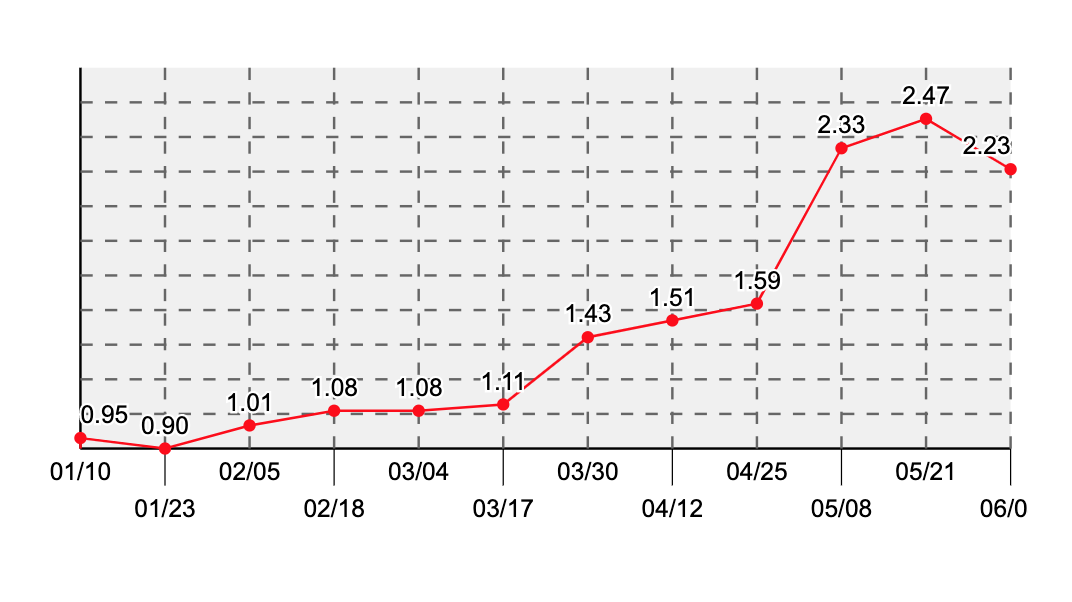
\includegraphics[width=\columnwidth]{../images/2019/zold-rate-june-2019.png}
    }
  \fact{zgreen}{Tech Audits}{%
    To help our potential clients better understand the value
    we can provide and less painfully migrate to the pay-by-result
    model of work and freelancers, we introduced a new product:
    \href{https://www.zerocracy.com/audits.html}{Tech Audits}. We already
    managed to sell a few audits and new requests are coming. We precict that
    many software teams and their CTOs/founders will be interested
    in independent technical reviews of their artifacts. Then, when
    a review is completed, it will be easier for them to move to
    \href{}{technical trainings} and then to fully integrating with Zerocracy.}
  \fact{zgreen}{GitHub Marketplace}{%
    We registered a few of our satellite applications, including
    \href{http://www.rultor.com}{Rultor} and \href{http://www.0pdd.com}{0pdd}
    at GitHub Marketplace, which makes them more visible for programmers
    and our potential customers. We are planning to register more of them
    there, including \href{https://www.0rsk.com}{0rsk}, \href{https://www.wring.io}{Wring},
    and others.}
\end{multicols}}

\slide{
  Facts
  \begin{multicols}{3}
  \fact{zblue}{Entity}{%
    Zerocracy, Inc.\\
    Delaware C-Corp}
  \fact{zblue}{Founded on}{%
    August 4, 2016}
  \fact{zblue}{Coordinates}{%
    555 Bryant, Ste 470\\
    CA 94301, USA\\
    408.692.4742\\
    \href{mailto:ceo@zerocracy.com}{ceo@zerocracy.com}}
  \fact{zblue}{Documents}{%
    \href{http://papers.zold.io/zerocracy-deck.pdf}{Pitch Deck}\\
    \href{http://papers.zold.io/executive-summary.pdf}{Executive Summary}\\
    \href{http://papers.zold.io/fin-model.pdf}{Fin Model} \\
    \href{http://papers.zold.io/offer.pdf}{Investment Offer} \\
    \href{http://papers.zold.io/features-deck.pdf}{Zerocrat Features} \\
    \href{http://papers.zold.io/freelance-deck.pdf}{Freelance Deck} \\
    \href{http://papers.zold.io/arc-deck.pdf}{Zerocracy Architecture} \\}
  \fact{zblue}{Business}{%
    Zerocracy is an AI-empowered project management chatbot that automates
    routine processes in software development projects, helping managers
    coordinate programmers in distributed and co-located teams.}
  \fact{zblue}{Social Networks}{%
    \href{https://github.com/zerocracy}{GitHub},
    \href{https://twitter.com/0crat}{Twitter},
    \href{https://www.facebook.com/zerocracy}{Facebook},
    \href{https://instagram.com/zerocracy}{Instagram},
    \href{https://www.linkedin.com/company/zerocracy}{LinkedIn}}
  \fact{zblue}{CEO}{%
    \href{https://www.yegor256.com/about-me.html}{Yegor Bugayenko} \\
    \href{https://twitter.com/intent/follow?screen_name=yegor256}{\includegraphics[height=1em]{../images/twitter.pdf}}
    \href{https://github.com/yegor256}{\includegraphics[height=1em]{../images/github.pdf}}
    \href{https://www.facebook.com/yegor256}{\includegraphics[height=1em]{../images/facebook.pdf}}
    \href{https://www.linkedin.com/in/yegor256}{\includegraphics[height=1em]{../images/linkedin.pdf}}}
  \fact{zblue}{Team}{%
    Erik J. Larson, PhD, Advisor\\
    \href{https://www.linkedin.com/in/erik-larson-b287ba9/}{\includegraphics[height=1em]{../images/linkedin.pdf}}

    Kiril Cherniavsky, Chief Architect\\
    \href{https://twitter.com/intent/follow?screen_name=kirill_g4s8}{\includegraphics[height=1em]{../images/twitter.pdf}}
    \href{https://github.com/g4s8}{\includegraphics[height=1em]{../images/github.pdf}}

    Carlos Miranda, Senior Developer\\
    \href{https://github.com/carlosmiranda}{\includegraphics[height=1em]{../images/github.pdf}}
    \href{https://www.linkedin.com/in/carlos-miguel-miranda-0b899392/}{\includegraphics[height=1em]{../images/linkedin.pdf}}

    Krzysztof Kraso\'n, Senior Deveoper\\
    \href{https://github.com/krzyk}{\includegraphics[height=1em]{../images/github.pdf}}
    \href{https://www.linkedin.com/in/krzyk/}{\includegraphics[height=1em]{../images/linkedin.pdf}}

    George Aristy, Senior Developer\\
    \href{https://github.com/llorllale}{\includegraphics[height=1em]{../images/github.pdf}}
    \href{https://www.linkedin.com/in/georgearisty/}{\includegraphics[height=1em]{../images/linkedin.pdf}}
    }
\end{multicols}}

\slide{
  Financials
  \begin{multicols}{3}
  \fact{zblue}{Shareholders}{%
    \renewcommand{\tabcolsep}{0pt}
    \begin{tabular}{l@{\hskip 6pt}r}
      Yegor Bugayenko & 80.60\% \\
      Erik J. Larson & 0.25\% \\
      Kiril Cherniavsky & 0.18\% \\
      Carlos Miranda & 0.07\% \\
      Others & 0.25\% \\
      Pool & 18.65\% \\
    \end{tabular}}
  \fact{zblue}{Total Shares}{%
    100,000,000}
  \fact{zblue}{Invested to Date}{%
    \$989,000 \up{+\$16K}}
  \fact{zblue}{Pre-Money Cap}{%
    \$16,000,000}
  \fact{zblue}{Raising Capital}{%
    \$400--1,600K}
  \fact{zblue}{Paying Customers}{%
    % January
    % Zold
    % Farm
    % Harvest
    % Stryvers
    5 }
  \fact{zblue}{Revenue /mo}}
  \fact{zblue}{Income /mo}}
  \fact{zblue}{Fixed Costs /mo}{%
    % Yegor $10k
    % AWS $300
    % Marketing guys: $400
    % Heroku: $400
    % Promo (buffer.com etc): $200
    \$11,300}
  \fact{zblue}{Sandbox Donations /mo}{%
    none }
  \fact{zblue}{Profit /mo}{% Income - FixedCost - Sandbox
    -\$9,210}
\end{multicols}

\large
All interval ``/mo'' metrics are related to the last calendar month.}

\slide{
  \begin{textblock}{2}[1,0](15,1)
    \includegraphics[height=64pt]{../images/zerocrat.pdf}
  \end{textblock}
  Zerocrat Tech Summary
  \begin{multicols}{3}
  \fact{zblue}{Version}{%
    \href{https://github.com/zerocracy/farm/releases}{0.47.5} \up{+7}\\
    Released on Jun-2 (two days ago)}
  \fact{zblue}{Top Programmers}}
  \fact{zblue}{Active Programmers}}
  \fact{zblue}{Total Reputation}}
  \fact{zblue}{Projects}}
  \fact{zblue}{Hits-of-code}{%
    \renewcommand{\tabcolsep}{0pt}
    \begin{tabular}{l@{\hskip 6pt}r}
      \href{https://github.com/zerocracy/farm}{zerocracy/farm} & 190K \\
      \href{https://github.com/zerocracy/datum}{zerocracy/datum} & 19K \\
      \href{https://github.com/yegor256/0pdd}{yegor256/0pdd} & 15K \\
      \href{https://github.com/yegor256/pdd}{yegor256/pdd} & 12K \\
    \end{tabular}}
\end{multicols}}

\slide{
  \begin{textblock}{2}[1,0](15,1)
    \includegraphics[height=64pt]{../images/logo.pdf}
  \end{textblock}
  Zold Cryptocurrency Tech/Fin Summary
  \begin{multicols}{3}
  \fact{zblue}{Version}{%
    \href{https://github.com/zold-io/zold/releases}{0.29.30} \up{+2}\\
    Released on 21-May (15 days ago)}
  \fact{zblue}{Total Emission}{%
    131,072}
  \fact{zblue}{Total Fund}}
  \fact{zblue}{Deficit}}
  \fact{zblue}{ZLD Rate}{%
    \href{https://wts.zold.io/rate}{0.0002812 BTC}}
  \fact{zblue}{ZLD Price}}
  \fact{zblue}{Nodes}}
  \fact{zblue}{Hits-of-code}{%
    \renewcommand{\tabcolsep}{0pt}
    \begin{tabular}{l@{\hskip 6pt}r}
      \href{https://github.com/zold-io/zold}{zold-io/zold} & 46K \\
      \href{https://github.com/zold-io/zold-stress}{zold-io/zold-stress} & 3K \\
      \href{https://github.com/zold-io/zold-score}{zold-io/zold-score} & 1K \\
      \href{https://github.com/zold-io/wts.zold.io}{zold-io/wts} & 11K \\
      \href{https://github.com/zold-io/zold.github.io}{zold-io/zold.github.io} & 32K \\
    \end{tabular}}
\end{multicols}}

\slide{
  Marketing and Promotion
  \begin{multicols}{3}
  \fact{zblue}{Active Users /mo} 1897 \\
      \href{https://www.zold.io}{zold.io} & \down{-5\%} 893 \\
    \end{tabular}}
  \fact{zblue}{Blog Posts}{%
    \renewcommand{\tabcolsep}{0pt}
    \begin{tabular}{l@{\hskip 6pt}r}
      \href{https://www.zerocracy.com/blog.html}{zerocracy.com/blog.html} & \up{+2} 18 \\
      \href{https://blog.zold.io}{blog.zold.io} & \up{+1} 31 \\
    \end{tabular}}
  \fact{zblue}{Social Followers} 719 \\
      \href{https://www.linkedin.com/company/zerocracy/}{LinkedIn} & 78 \\
      \href{https://www.youtube.com/channel/UCxZAzmY_OPw40I1-YStWqhw}{YouTube} & \up{+18\%} 135 \\
    \end{tabular}}
  \fact{zblue}{GitHub Stars}}
  \fact{zblue}{Website Leads /mo}}
  \fact{zblue}{Conferences /mo}{%
    \emph{QualityConf}, Moscow, Russia
    % BeeMobile Meetup, Moscow, Russia\\
  }
  \end{multicols}

  \large All interval ``/mo'' metrics are related to the last calendar month.
}

\tailslide

\end{document}
